\documentclass[14pt]{extbook}
\usepackage{multicol, enumerate, enumitem, hyperref, color, soul, setspace, parskip, fancyhdr} %General Packages
\usepackage{amssymb, amsthm, amsmath, bbm, latexsym, units, mathtools} %Math Packages
\everymath{\displaystyle} %All math in Display Style
% Packages with additional options
\usepackage[headsep=0.5cm,headheight=12pt, left=1 in,right= 1 in,top= 1 in,bottom= 1 in]{geometry}
\usepackage[usenames,dvipsnames]{xcolor}
\usepackage{dashrule}  % Package to use the command below to create lines between items
\newcommand{\litem}[1]{\item#1\hspace*{-1cm}\rule{\textwidth}{0.4pt}}
\pagestyle{fancy}
\lhead{Makeup Progress Quiz 1}
\chead{}
\rhead{Version C}
\lfoot{6018-3080}
\cfoot{}
\rfoot{Spring 2021}
\begin{document}

\begin{enumerate}
\litem{
Solve the radical equation below. Then, choose the interval(s) that the solution(s) belongs to.\[ \sqrt{-5 x + 4} - \sqrt{-6 x - 8} = 0 \]\begin{enumerate}[label=\Alph*.]
\item \( \text{All solutions lead to invalid or complex values in the equation.} \)
\item \( x_1 \in [-13, -10] \text{ and } x_2 \in [0.8,3.8] \)
\item \( x \in [-13,-10] \)
\item \( x \in [1,10] \)
\item \( x_1 \in [-4.33, -0.33] \text{ and } x_2 \in [0.8,3.8] \)

\end{enumerate} }
\litem{
What is the domain of the function below?\[ f(x) = \sqrt[5]{8 x - 5} \]\begin{enumerate}[label=\Alph*.]
\item \( \text{The domain is } (-\infty, a], \text{   where } a \in [1.55, 1.8] \)
\item \( \text{The domain is } (-\infty, a], \text{   where } a \in [0.15, 1.5] \)
\item \( \text{The domain is } [a, \infty), \text{   where } a \in [1, 2.4] \)
\item \( \text{The domain is } [a, \infty), \text{   where } a \in [-0.3, 0.9] \)
\item \( (-\infty, \infty) \)

\end{enumerate} }
\litem{
Choose the graph of the equation below.\[ f(x) = - \sqrt[3]{x + 10} + 4 \]\begin{enumerate}[label=\Alph*.]
\begin{multicols}{2}\item 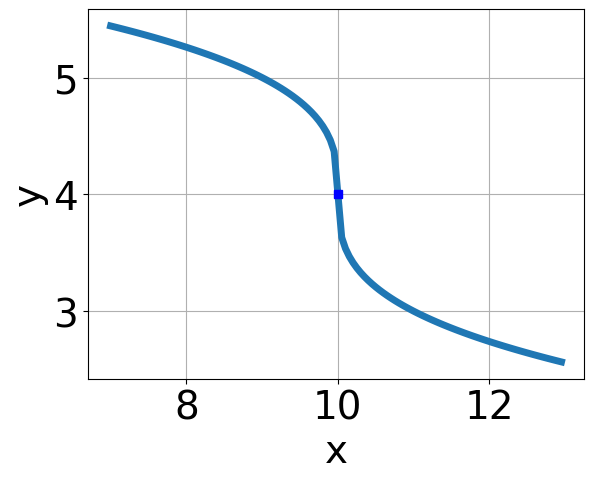
\includegraphics[width = 0.3\textwidth]{../Figures/radicalEquationToGraphAC.png}\item 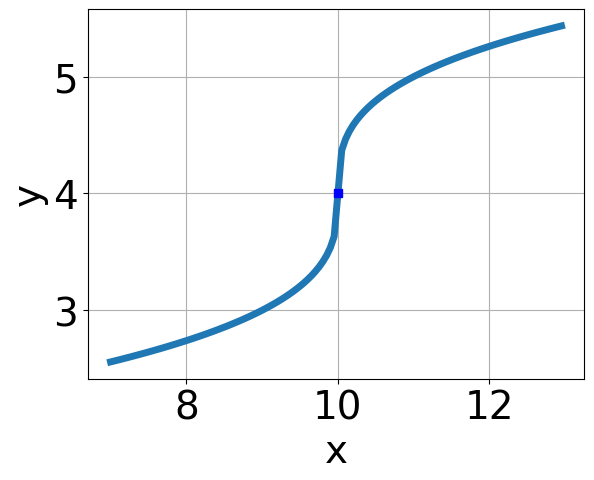
\includegraphics[width = 0.3\textwidth]{../Figures/radicalEquationToGraphBC.png}\item 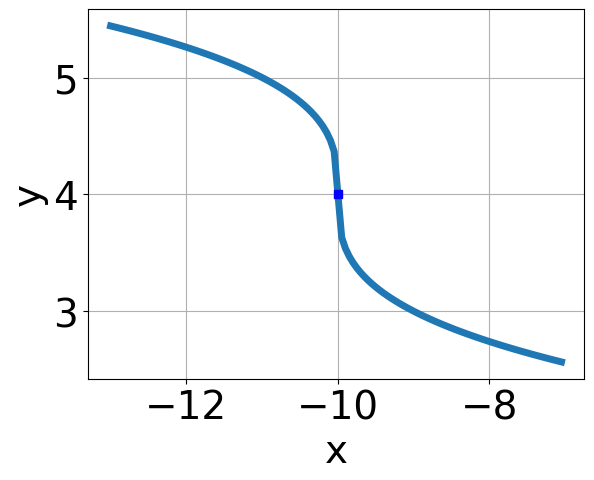
\includegraphics[width = 0.3\textwidth]{../Figures/radicalEquationToGraphCC.png}\item 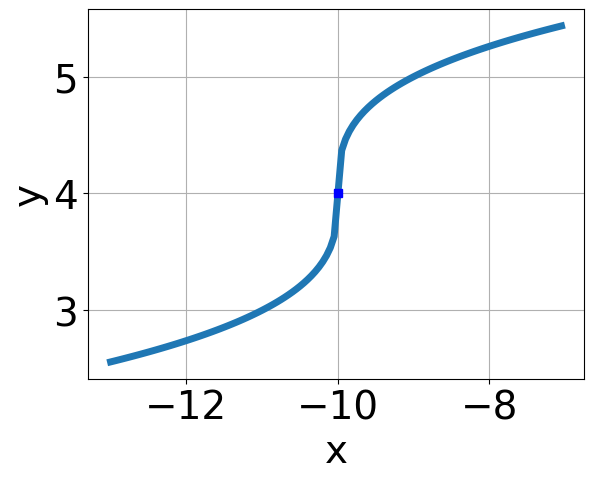
\includegraphics[width = 0.3\textwidth]{../Figures/radicalEquationToGraphDC.png}\end{multicols}\item None of the above.
\end{enumerate} }
\litem{
Solve the radical equation below. Then, choose the interval(s) that the solution(s) belongs to.\[ \sqrt{35 x^2 + 81} - \sqrt{108 x} = 0 \]\begin{enumerate}[label=\Alph*.]
\item \( x_1 \in [-1.97, -1.49] \text{ and } x_2 \in [-1.29,-0.29] \)
\item \( x_1 \in [1.16, 1.48] \text{ and } x_2 \in [-1.2,3.8] \)
\item \( \text{All solutions lead to invalid or complex values in the equation.} \)
\item \( x \in [1.65,1.94] \)
\item \( x \in [1.16,1.48] \)

\end{enumerate} }
\litem{
Choose the equation of the function graphed below.
\begin{center}
    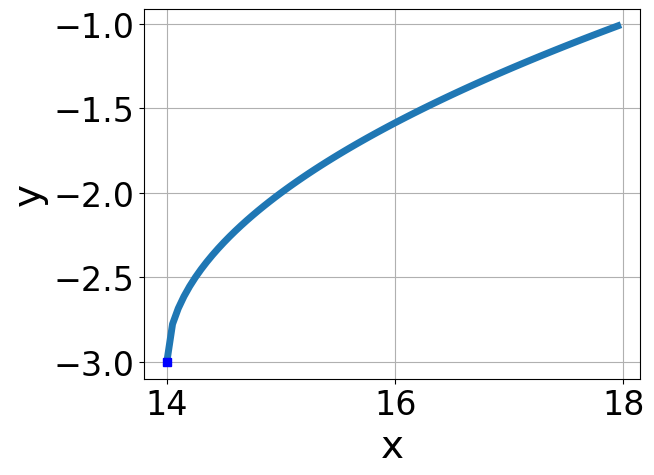
\includegraphics[width=0.5\textwidth]{../Figures/radicalGraphToEquationCopyC.png}
\end{center}
\begin{enumerate}[label=\Alph*.]
\item \( f(x) = \sqrt{x - 14} - 3 \)
\item \( f(x) = \sqrt{x + 14} - 3 \)
\item \( f(x) = - \sqrt{x - 14} - 3 \)
\item \( f(x) = - \sqrt{x + 14} - 3 \)
\item \( \text{None of the above} \)

\end{enumerate} }
\litem{
What is the domain of the function below?\[ f(x) = \sqrt[4]{4 x - 6} \]\begin{enumerate}[label=\Alph*.]
\item \( (-\infty, a], \text{where } a \in [0.7, 4.5] \)
\item \( (-\infty, a], \text{where } a \in [-1.8, 1.3] \)
\item \( (-\infty, \infty) \)
\item \( [a, \infty), \text{where } a \in [0.01, 1.42] \)
\item \( [a, \infty), \text{ where } a \in [0.85, 3.18] \)

\end{enumerate} }
\litem{
Solve the radical equation below. Then, choose the interval(s) that the solution(s) belongs to.\[ \sqrt{-28 x^2 - 27} - \sqrt{75 x} = 0 \]\begin{enumerate}[label=\Alph*.]
\item \( x_1 \in [1.7, 4.6] \text{ and } x_2 \in [0.17,1.28] \)
\item \( x \in [-4.5,-1.8] \)
\item \( \text{All solutions lead to invalid or complex values in the equation.} \)
\item \( x_1 \in [-4.5, -1.8] \text{ and } x_2 \in [-0.97,-0.23] \)
\item \( x \in [-1.5,-0.2] \)

\end{enumerate} }
\litem{
Choose the equation of the function graphed below.
\begin{center}
    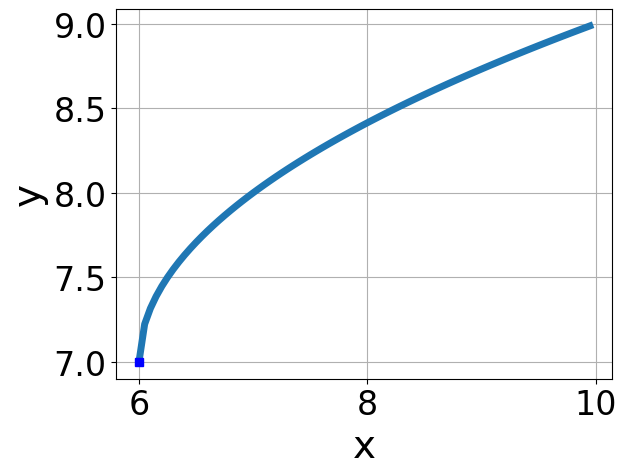
\includegraphics[width=0.5\textwidth]{../Figures/radicalGraphToEquationC.png}
\end{center}
\begin{enumerate}[label=\Alph*.]
\item \( f(x) = - \sqrt[3]{x - 6} + 7 \)
\item \( f(x) = - \sqrt[3]{x + 6} + 7 \)
\item \( f(x) = \sqrt[3]{x - 6} + 7 \)
\item \( f(x) = \sqrt[3]{x + 6} + 7 \)
\item \( \text{None of the above} \)

\end{enumerate} }
\litem{
Solve the radical equation below. Then, choose the interval(s) that the solution(s) belongs to.\[ \sqrt{7 x - 3} - \sqrt{3 x + 7} = 0 \]\begin{enumerate}[label=\Alph*.]
\item \( x_1 \in [-0.37, 0.66] \text{ and } x_2 \in [0.7,4.2] \)
\item \( x \in [-1.31,-0.01] \)
\item \( x \in [1.41,2.96] \)
\item \( x_1 \in [-2.53, -1.69] \text{ and } x_2 \in [-0.1,1.7] \)
\item \( \text{All solutions lead to invalid or complex values in the equation.} \)

\end{enumerate} }
\litem{
Choose the graph of the equation below.\[ f(x) = - \sqrt[3]{x + 6} - 6 \]\begin{enumerate}[label=\Alph*.]
\begin{multicols}{2}\item 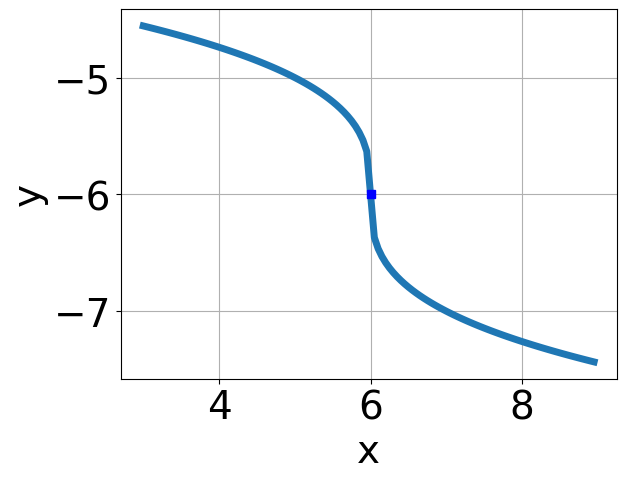
\includegraphics[width = 0.3\textwidth]{../Figures/radicalEquationToGraphCopyAC.png}\item 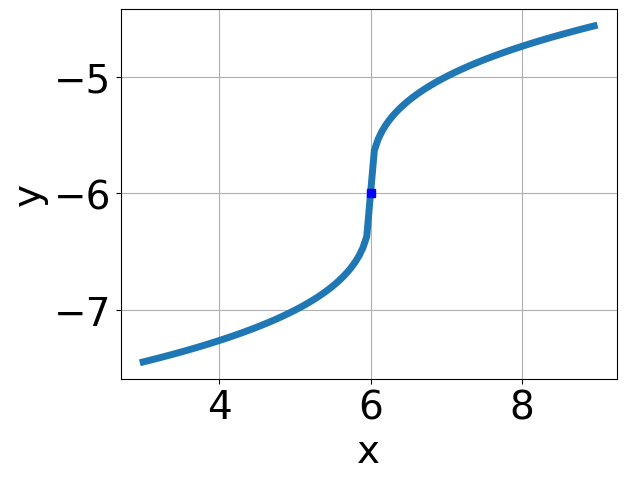
\includegraphics[width = 0.3\textwidth]{../Figures/radicalEquationToGraphCopyBC.png}\item 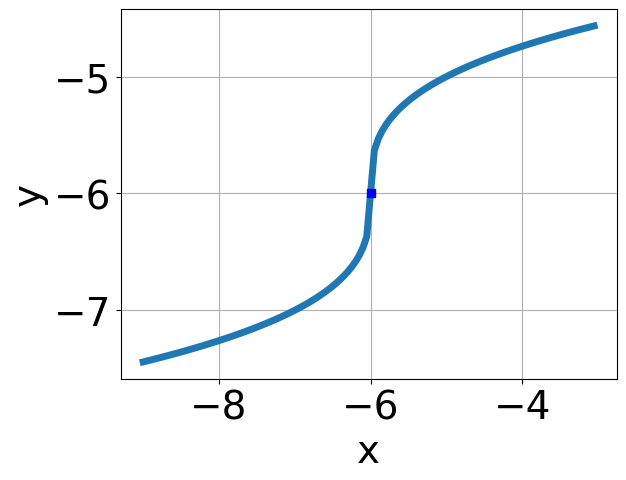
\includegraphics[width = 0.3\textwidth]{../Figures/radicalEquationToGraphCopyCC.png}\item 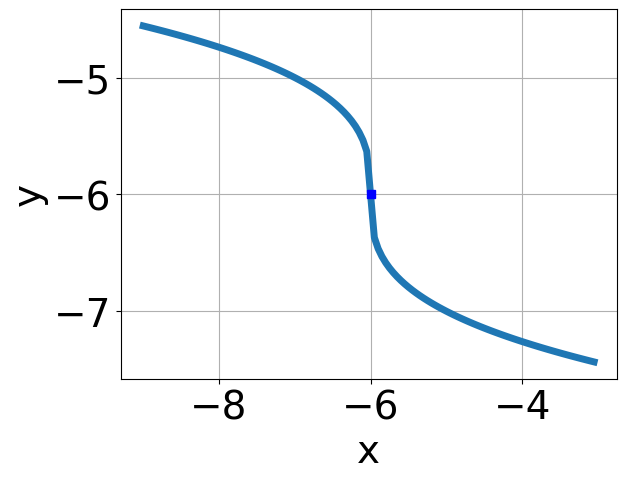
\includegraphics[width = 0.3\textwidth]{../Figures/radicalEquationToGraphCopyDC.png}\end{multicols}\item None of the above.
\end{enumerate} }
\end{enumerate}

\end{document}